% Description of the paper meetings and their explanation

\section{Meetings}
Retaining the exact same number of players, each generation, requires rounding up the emerging number of players each strategy has at the end of each generation and then redistributing the decimal parts. Ultimately, the decimal parts in our 3-strategy meetings add up to either one or two, and the distribution method we found to be the most fair was:
\begin{itemize}
    \item If the remainder sum is 1, we round up each strategy to the previous integer and distribute the decimal part to the strategy that is the closest to its next integer.
    \item If the remainder sum is 2, we round up each strategy to the previous integer and distribute the decimal part to the two strategies that are the closest to their next integer. 1 to each.
    \item If the remainder sum is 0, there are no decimal parts.
\end{itemize}
We also devised a similar method which this time distributes the decimal parts to the top two strategies in terms of total population. We used the first of the two, ("dec"), to conduct our experiments. However, when comparing our results with the 1999's paper "Studies on Dynamics in the Classical Iterated Prisoner's Dilemma with Few Strategies" the graphs we produced were mostly coherent but ultimately different. These differences can be largely attributed to the mutable nature of the simulations hidden in programming layers of abstraction and the non-disclosed method of rounding used by the authors of the paper. They only stated that: "All divisions being rounded to the nearest lower integer.", which is not accurate based on their results which seem to be retaining their initial total population. This will be an attempt to replicate the paper's results while attributing our differences and trying to make the same point the original authors were trying to make regardless of the differences. Here is our rounding logic: 
\begin{}
%%%%%%%% DECIMAL REDISTRIBUTION %%%%%%%%%%%%%
if rounding == "pop"
    remainder = zeros(1, length(strategies));

    for i = 1:length(strategies)
        Wn(i) = totalplayers * Gn(i)*Wn(i) / Tn;
        remainder(i) = Wn(i) - floor(Wn(i));
        Wn(i) = floor(Wn(i));
    end

    remaining = totalplayers - sum(Wn);  % How many individuals to redistribute
    [~, sortedIndices] = sort(Wn, 'descend');  % Sort by largest populations

    for k = 1:remaining
        Wn(sortedIndices(k)) = Wn(sortedIndices(k)) + 1;
    end
end
if rounding == "dec"
    remainder = zeros(1, length(strategies));

    for i = 1:length(strategies)
        Wn(i) = totalplayers * Gn(i) * Wn(i) / Tn;
        remainder(i) = Wn(i) - floor(Wn(i));
        Wn(i) = floor(Wn(i));
    end

    remaining = totalplayers - sum(Wn);  % How many individuals to redistribute
    [~, sortedIndices] = sort(remainder, 'descend');  % Sort by largest decimals

    for k = 1:remaining
        Wn(sortedIndices(k)) = Wn(sortedIndices(k)) + 1;
    end
end            
if rounding == "off"
    for i = 1:length(strategies)
        Wn(i) = totalplayers * Gn(i)*Wn(i) / Tn;
    end
end
\end{}
It is important to note that when comparing equal quantities the is no clear ranking between remainders. Thus the program decides where to distribute the decimal parts based on the order of the strategies. This could very well be consequential enough to skew the results in a different direction. Let's see how our results compare relative to the ones in the paper.

\subsection{Defectors may be strong}
This meeting is supposed to show how defecting more often can be beneficial in chaotic environments. WHen rounding using the "dec method we observe oscillations that converge to a stable state. 
\begin{figure}[H]
    \centering
    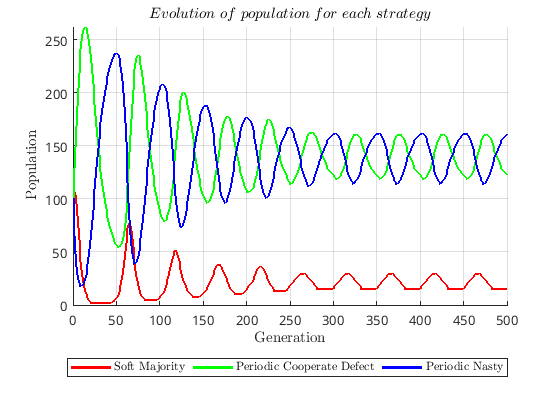
\includegraphics[width=0.8\textwidth]{media/meetings/defectors_may_be_strong_dec.png}
    \caption{Defectors may be strong Dec Plot}
\end{figure}
When rounding using the "pop" method we replicate the results of the paper.
\begin{figure}[H]
    \centering
    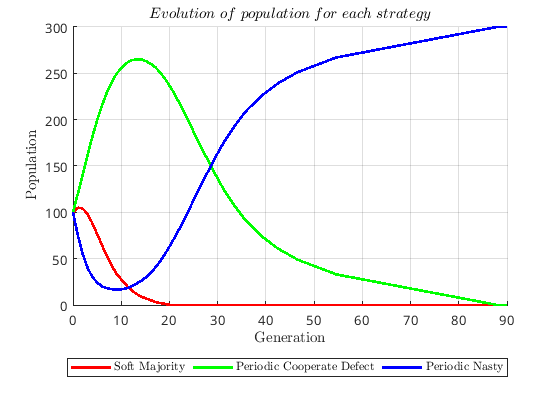
\includegraphics[width=0.8\textwidth]{media/meetings/defectors_may_be_strong_pop.png}
    \caption{Defectors may be strong Pop Plot}
\end{figure}

\subsection{Monotonous convergence}
This meeting simulates clear monotonous convergence. The paper claims this is the most common outcome of the experiments they ran. Here both "pop" and "dec" methods produced identical results recreating the paper's plots. 
\begin{figure}[H]
    \centering
    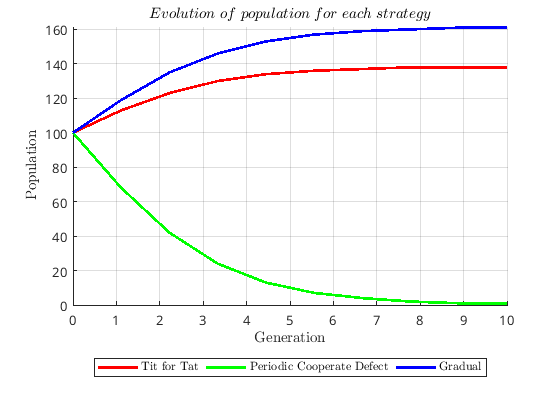
\includegraphics[width=0.8\textwidth]{media/meetings/monotonous_convergence_dec.png}
    \caption{Monotonous convergence Plot}
\end{figure}

\subsection{Attenuated oscillatory movements}
Here we see decreasing oscillations that reach an equilibrium. Both rounding methods are again very close to the paper.
\begin{figure}[H]
    \centering
    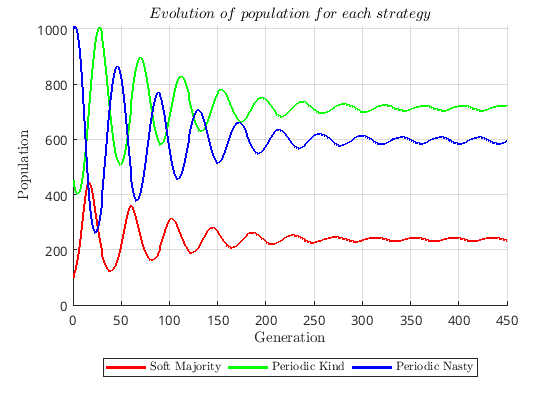
\includegraphics[width=0.8\textwidth]{media/meetings/attenuated_oscillatory_movements_dec.png}
    \caption{Attenuated oscillatory movements Plot}
\end{figure}

\subsection{Periodic movements}
The periodic movements meeting highlights the periodicity and constant amplitude of the oscillations but changing the rounding method changes the amplitude.
\begin{figure}[H]
    \centering
    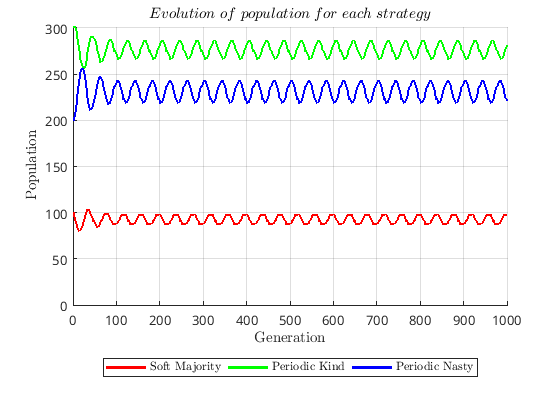
\includegraphics[width=0.8\textwidth]{media/meetings/periodic_movements_dec.png}
    \caption{Periodic movements Plot}
\end{figure}
Increased amplitude in "pop" method.
\begin{figure}[H]
    \centering
    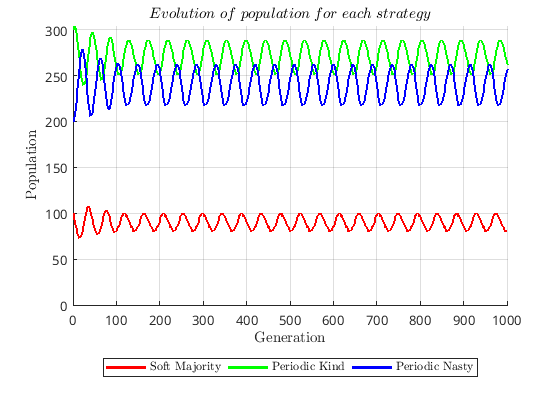
\includegraphics[width=0.8\textwidth]{media/meetings/periodic_movements_pop.png}
    \caption{Periodic movements Pop Plot}
\end{figure}

\subsection{Increasing oscillations}
We were unable to replicate these results. The oscillations seem to converge in all three rounding methods we used.
\begin{figure}[H]
    \centering
    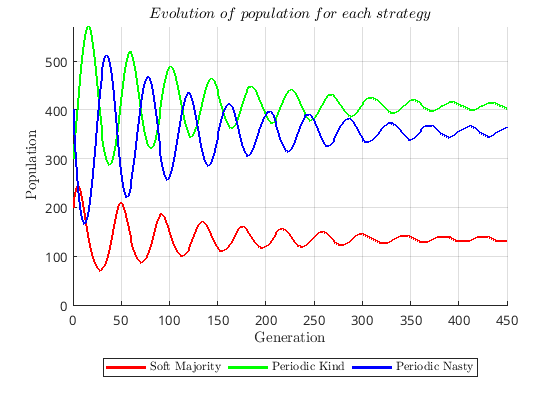
\includegraphics[width=0.8\textwidth]{media/meetings/increasing_oscillations_dec.png}
    \caption{Increasing oscillations Plot}
\end{figure}

\subsection{Disordered oscillations}
When examining the disordered oscillations, the closest we could get was the "off" method. However the phenomenon ended quicker, at around 260 generations and the final state had soft majority and periodic ultra kind strategies go extinct. "dec" and "pop" had very similar behaviour to the attenuated oscillatory movements meeting.
\begin{figure}[H]
    \centering
    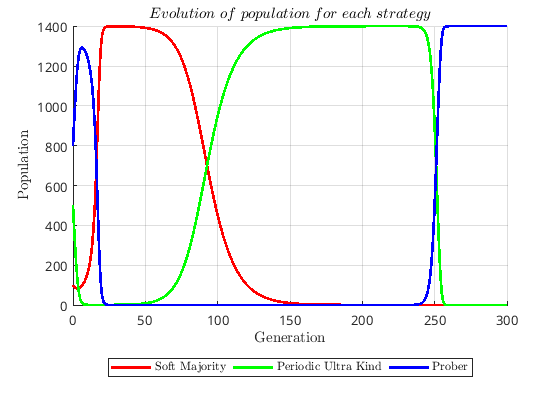
\includegraphics[width=0.8\textwidth]{media/meetings/disordered_oscillations_off.png}
    \caption{Disordered oscillations off Plot}
\end{figure}

\subsection{Population size sensitivity}
Going forward the paper decides to explore the tournament's sensitivity to various parameters starting with initial population size.
\begin{figure}[H]
    \centering
    \includegraphics[width=0.8\textwidth]{media/meetings/population_size_sensitivity.png}
    \caption{Population size sensitivity before Plot}
\end{figure}
\begin{figure}[H]
    \centering
    \includegraphics[width=0.8\textwidth]{media/meetings/population_size_sensitivity_after.png}
    \caption{Population size sensitivity after Plot}
\end{figure}

\subsection{Population size sensitivity 2}
\begin{figure}[H]
    \centering
    \includegraphics[width=0.8\textwidth]{media/meetings/population_size_sensitivity_2.png}
    \caption{Population size sensitivity 2 before Plot}
\end{figure}
\begin{figure}[H]
    \centering
    \includegraphics[width=0.8\textwidth]{media/meetings/population_size_sensitivity_2_after.png}
    \caption{Population size sensitivity 2 after Plot}
\end{figure}

\subsection{Game length sensitivity}
\begin{figure}[H]
    \centering
    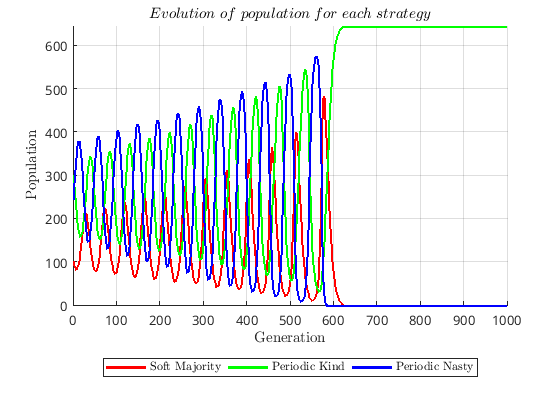
\includegraphics[width=0.8\textwidth]{media/meetings/game_length_sensitivity_before.png}
    \caption{Game length sensitivity before Plot}
\end{figure}
\begin{figure}[H]
    \centering
    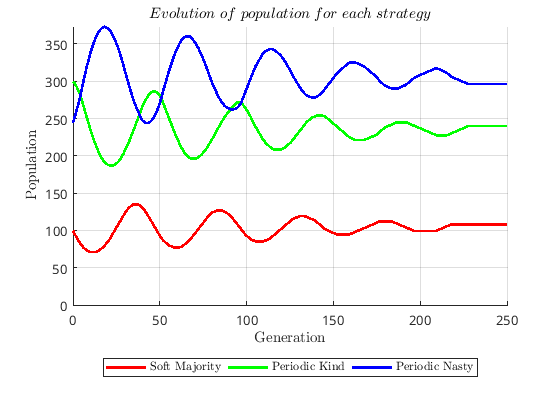
\includegraphics[width=0.8\textwidth]{media/meetings/game_length_sensitivity_after.png}
    \caption{Game length sensitivity after Plot}
\end{figure}

\subsection{Payoff matrix sensitivity}
\begin{figure}[H]
    \centering
    \includegraphics[width=0.8\textwidth]{media/meetings/payoff_matrix_sensitivity.png}
    \caption{Payoff matrix sensitivity before Plot}
\end{figure}
\begin{figure}[H]
    \centering
    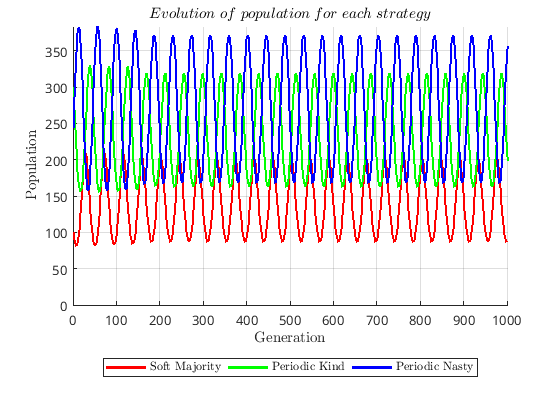
\includegraphics[width=0.8\textwidth]{media/meetings/payoff_matrix_sensitivity_after.png}
    \caption{Payoff matrix sensitivity after Plot}
\end{figure}

\subsection{Rounding method sensitivity}
\begin{figure}[H]
    \centering
    \includegraphics[width=0.8\textwidth]{media/meetings/rounding_method_sensitivity.png}
    \caption{Rounding method sensitivity before Plot}
\end{figure}
\begin{figure}[H]
    \centering
    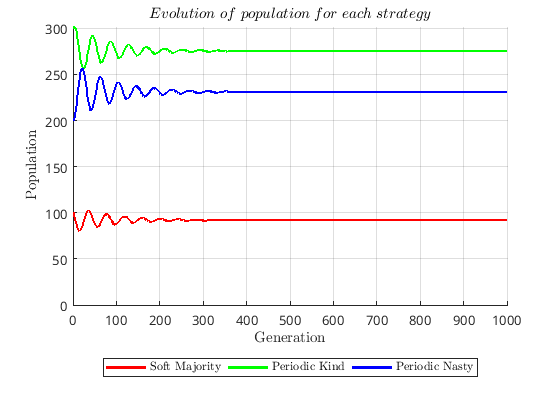
\includegraphics[width=0.8\textwidth]{media/meetings/rounding_method_sensitivity_after.png}
    \caption{Rounding method sensitivity after Plot}
\end{figure}
\begin{figure}[H]
    \centering
    \includegraphics[width=0.8\textwidth]{media/meetings/rounding_method_sensitivity_2.png}
    \caption{Rounding method sensitivity 2 before Plot}
\end{figure}
\begin{figure}[H]
    \centering
    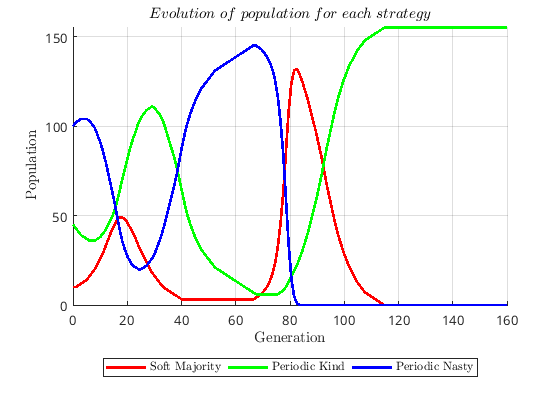
\includegraphics[width=0.8\textwidth]{media/meetings/rounding_method_sensitivity_2_after.png}
    \caption{Rounding method sensitivity 2 after Plot}
\end{figure}

